\documentclass[12pt,letterpaper,titlepage]{article}
\usepackage{solarized-light}
\usepackage{fontspec}
\defaultfontfeatures{Mapping=tex-text}
\usepackage{xunicode}
\usepackage{xltxtra}
\usepackage{amsmath}
\usepackage{pdfpages}
\usepackage{amsfonts}
\usepackage{amssymb}
\setcounter{secnumdepth}{0}
\usepackage{nameref}
\usepackage{enumitem}
\usepackage{environ}
\usepackage[pdf]{graphviz}
\usepackage{pdfpages}
\usepackage{pgfplots}
\usepackage{karnaugh-map}

\setmainfont{Times New Roman}
\showboxdepth=\maxdimen
\showboxbreadth=\maxdimen


\usepackage{paracol}
\usepackage{wrapfig}
\globalcounter{table}
\globalcounter{figure}
\usepackage{graphicx}
\usepackage[left=1in,right=1in,top=1in,bottom=1in]{geometry}
\graphicspath{{img/}}

\author{Jacob Abel}
\title{	Project 5
	\\\large ECE3544 CRN:82989
}

\setlength{\parskip}{0.25em}

\begin{document}
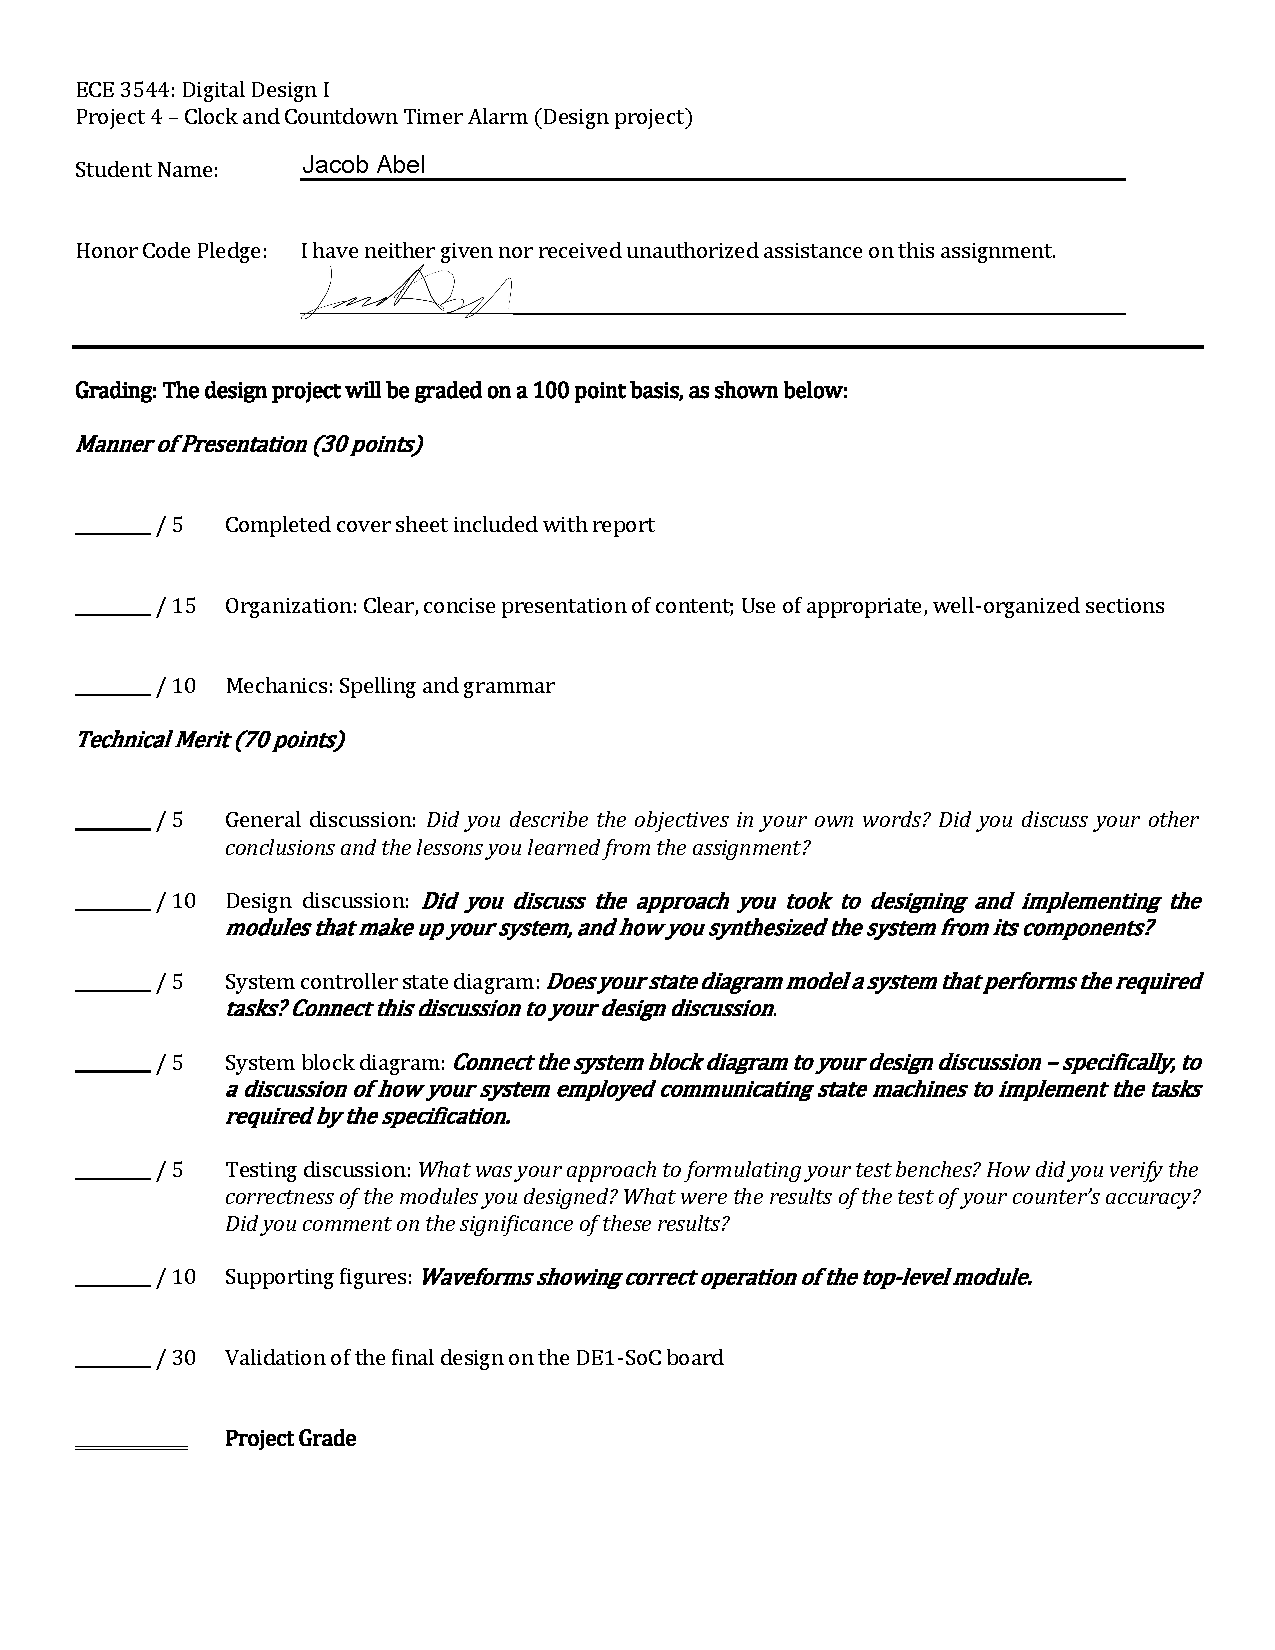
\includepdf[noautoscale]{CoverSheet.pdf}
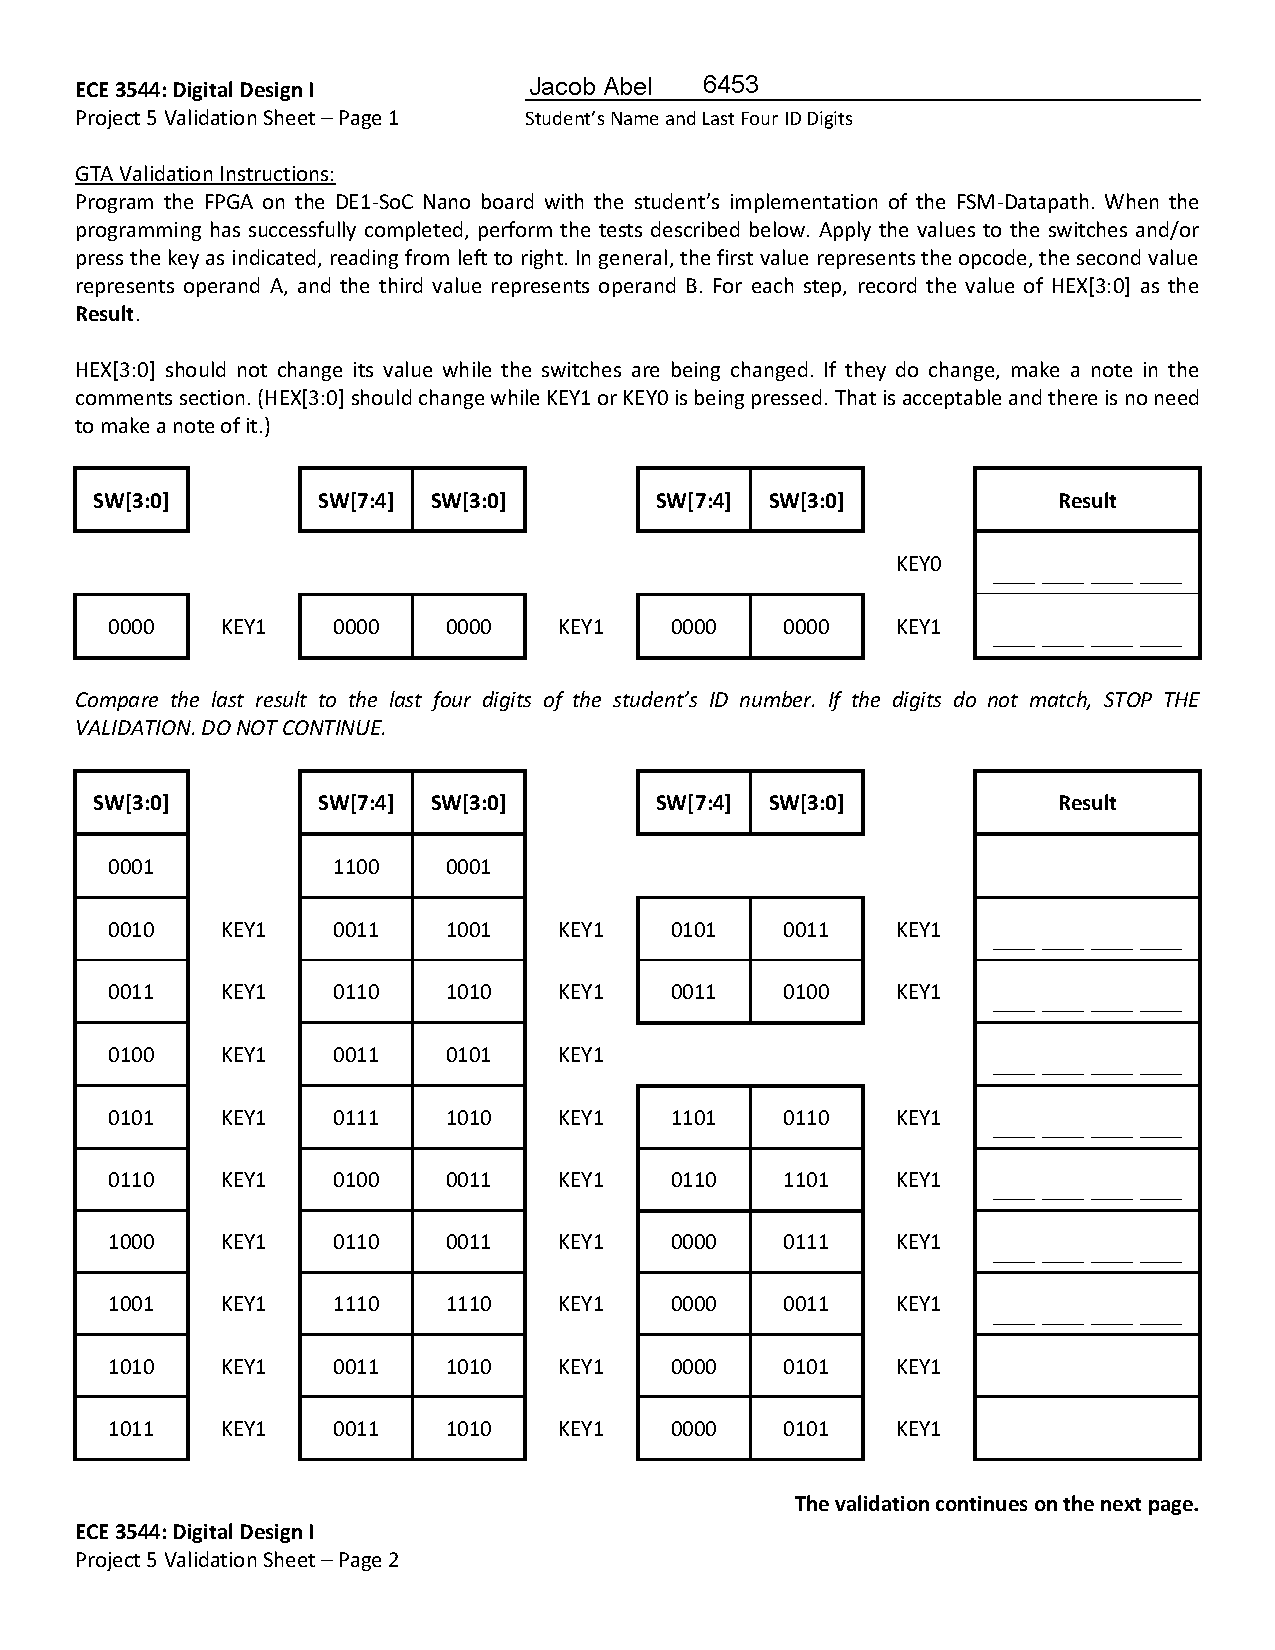
\includepdf[noautoscale]{ValidationSheet.pdf}

\maketitle
\begin{raggedright}

\section*{Objective}

\section{Primary Control FSM Diagram}


\section{FSM Module Design}


\clearpage
\section{Project FSM Module Simulation}

\section{Conclusion}

Unfortunately while the project was very pleasant to attempt, due to scheduling issues the final deliverable is largely non functional.

\end{raggedright}
\end{document}
